      
               
                \begin{ledgroupsized}[r]{120mm}
                \footnotesize 
                \pstart                
                \noindent\textbf{\"{U}berlieferung:}   
                \pend
                \end{ledgroupsized}
            
              
                            \begin{ledgroupsized}[r]{114mm}
                            \footnotesize 
                            \pstart \parindent -6mm
                            \makebox[6mm][l]{\textit{L}}Notizen: LH XXXV 3A, 8 Bl. 27. 1 Bl. 20 x 21 cm, 1 S., R\"{u}ckseite mit Rechnungen und Zeichnungen zur Rechenmaschine, die in einem separaten Band mit den Texten zur Leibniz'schen Rechenmaschine gedruckt werden. Linke und untere Seite beschnitten. Links etwa in der Mitte noch einmal ein Rechteck von 2 x 9 cm herausgeschnitten. Die Zeichnung befindet sich in der rechten unteren Ecke.\\Cc 2, Nr. 282 \pend
                            \end{ledgroupsized}
                %\normalsize
                \vspace*{5mm}
                \begin{ledgroup}
                \footnotesize 
                \pstart
            \noindent\footnotesize{\textbf{Datierungsgr\"{u}nde}: Bei dem mittleren Teil des Textes handelt sich offenbar um Gespr\"{a}chsnotizen, in denen Details zum Inhalt der von Mariotte\protect\index{Namensregister}{\textso{Mariotte,} Edme, Seigneur de Chazeuil ca. 1620\textendash 1684} geplanten Schrift \cite{00186}\textit{De la nature des couleurs} mitgeteilt werden. Leibniz hat Mariotte im Fr\"{u}hjahr 1673 in Paris pers\"{o}nlich kennengelernt, so dass die Aufzeichnungen erst danach entstanden sein k\"{o}nnen. Ein Entstehungsdatum kurz nach dieser Unterredung wird durch das Wasserzeichen des benutzten Papiers gest\"{u}tzt, das f\"{u}r die 2. H\"{a}lfte 1672 sowie die 1. H\"{a}lfte 1673 belegt ist. Der Text wird daher zwischen Fr\"{u}hjahr und Sommer 1673 entstanden sein.}
                \pend
                \end{ledgroup}
            
                \vspace*{8mm}
                \pstart 
                \normalsize
            [27 r\textsuperscript{o}] Instrument pour Niveller\protect\index{Sachverzeichnis}{instrument pour niveller} avec une boule d'air.\pend \pstart Hubin\protect\index{Namensregister}{\textso{Hubin,} Ludion de } a fait un petit homme, quand l'eau est press\'{e}e \edtext{l'air dans}{\lemma{press\'{e}e}\Afootnote{ \textit{ (1) }\ l'eau dans \textit{ (2) }\ l'air dans \textit{ L}}} cet homme est press\'{e} aussi, et l'eau entre plus avant  dedans. Ainsi il devient pesant et tombe, en retirant l'eau par  force, il ressort et remonte, autrement non. Le doigt doit entrer justement.  Il a fait l'enfer, et le ciel, je luy appris aussi  \`{a} faire le \textso{purgatoire au milieu }\edtext{c'est par deux liqueurs l'une sur l'autre}{\lemma{}\Afootnote{ c'est par deux liqueurs  \textit{ (1) }\ de \textit{ (2) }\ sur la \textit{ (3) }\ l'une sur l'autre \textit{ erg.} \textit{ L}}}.\pend \pstart Thermometre de Florence\protect\index{Sachverzeichnis}{Thermom\`{e}tre de Florence}, huict Boules, pour la froideur, et 4. pour la chaleur\protect\index{Sachverzeichnis}{chaleur}, parce qu'il y a plus de froideur\protect\index{Sachverzeichnis}{froideur} aupres de nous que de chaleur\protect\index{Sachverzeichnis}{chaleur}. Mais ainsi on n'a que \edtext{12}{\lemma{que}\Afootnote{ \textit{ (1) }\ huict \textit{ (2) }\ 12 \textit{ L}}} degr\'{e}s seulement, c'est peu.  Man mus haben soviel blaßen als degre, c'est Bagatelle\edtext{, aber man kans auch besser machen.}{\lemma{}\Afootnote{, c'est [...] machen. \textit{ erg.} \textit{ L}}}  Man m\"{u}ste vielmehr machen daß eine Boule bald so weit auff, bald so weit absteige, nach der invention Mons. Boyle\protect\index{Namensregister}{\textso{Boyle} (Boylius, Boyl., Boyl), Robert 1627\textendash 1691}, das eine Boule fallet, wenn man mehr wasser drauff giesset, oder wenn sie tieffer. M. l'Abb\'{e} Mariotte\protect\index{Namensregister}{\textso{Mariotte,} Edme, Seigneur de Chazeuil ca. 1620\textendash 1684} publiera un trait\'{e} de perspective\protect\index{Sachverzeichnis}{perspective}, ce sera la 7\textsuperscript{me} partie de son \textit{optique}\edtext{}{\lemma{son}\Bfootnote{\textsc{E. Mariotte}, \cite{00186}\textit{De la nature des couleurs}, Paris 1681.}} Il cherche sur tout le point d'oil \textit{[!]}, dont il tire toutes les autres, dont l'intersection represente tout. Ducit in Tabulam lineam parallelam lineis rei  designandae, haec cadit in punctum visus etc.\pend \pstart Arc en ciel\protect\index{Sachverzeichnis}{arc en ciel} \edtext{}{\lemma{etc.}\Bfootnote{\textsc{E. Mariotte}, \cite{00186}a.a.O., Teil X.}} de M. l'Abb\'{e} Mariotte. Il sera publi\'{e} bien tost. Il y rend raison de tout par des Experiences. Il prend un tuyau de verre met au bas du vif argent\protect\index{Sachverzeichnis}{vif argent} sur cela du papier sur le papier de l'eau, le rayon \edtext{petit du soleil\protect\index{Sachverzeichnis}{soleil} entrant par un trou laiss\'{e} ouuert dans une chambre ferm\'{e}e}{\lemma{}\Afootnote{petit \protect\index{Sachverzeichnis}{soleil} [...] ferm\'{e}e \textit{ erg.} \textit{ L}}} tombant sur le papier le peint en divers couleurs\protect\index{Sachverzeichnis}{couleur}, principalement bleu et rouge. Ostez le papier laissez le vif argent\protect\index{Sachverzeichnis}{vif argent}, et l'eau, il se reflechira, \`{a} cause du vif argent\protect\index{Sachverzeichnis}{vif argent} qui l'empeche de passer, et on voit le rayon\protect\index{Sachverzeichnis}{rayon} reflechi sans couleurs\protect\index{Sachverzeichnis}{couleur}, car tout est remis. Il prend  au lieu de l'argent vif\protect\index{Sachverzeichnis}{vif argent} un miroir\protect\index{Sachverzeichnis}{miroir} et inclin\'{e} \`{a} sa volont\'{e}. Si l'angle  de l'incidence\protect\index{Sachverzeichnis}{angle!d'incidence}\protect\index{Sachverzeichnis}{angle!d'incidence|see{angolo di incidenza}}\protect\index{Sachverzeichnis}{angle!d'incidence|see{angulus incidentiae}}  et reflexion\protect\index{Sachverzeichnis}{angle!de r\'{e}flexion}\protect\index{Sachverzeichnis}{angle!de r\'{e}flexion|see{angulus reflexionis}} est \'{e}gal, il n'y a point de couleur, si le miroir\protect\index{Sachverzeichnis}{miroir} est inclin\'{e}  l'angle n'est pas \'{e}gal, et voila les couleurs\protect\index{Sachverzeichnis}{couleur}\protect\index{Sachverzeichnis}{couleur|see{color}} couleur, bleu rouge, bleu rouge, bleu rouge; rien, rouge bleu, rouge bleu, rouge bleu, de l'autre cost\'{e}.\pend \pstart Instrument \`{a} Niveller\protect\index{Sachverzeichnis}{instrument pour niveller}. Versez de l'eau \edtext{sur une planche longue couuerte}{\lemma{l'eau}\Afootnote{ \textit{ (1) }\ dans un long cana \textit{ (2) }\ sur une planche longue couuerte \textit{ L}}}
              \begin{wrapfigure}{l}{0.3\textwidth}                    
              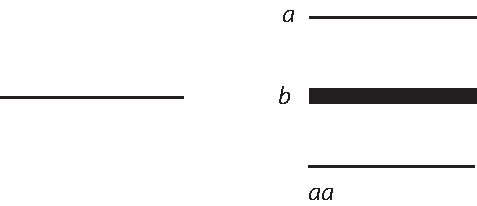
\includegraphics[width=0.3\textwidth]{images/35_3A_8_27r}
              \\\centering\textit{[Fig. 1]}
              \end{wrapfigure}
            de costez, ouuerte par avant et par derriere, la cire empeche l'eau  de ne sortir pas. Regardez l'objet prenez deux \edtext{points dedans, \textit{a} et \textit{b}}{\lemma{deux}\Afootnote{ \textit{ (1) }\ parties dedans, si vous \textit{ (2) }\ points dedans, \textit{a} et \textit{b} \textit{ L}}} les  haussez et baissez si long temps, jusqu'\`{a} ce qu' \textit{a} se represente in \textit{aa} infra \textit{b} in aqua, in eadem  distantia, ut \textit{a} est supra \textit{b} ita \textit{aa} erit infra \textit{b}.\pend 